%%%%%%%%%%%%%%%%%%%%%%%%%%%%%%%%%%%%%%%%%%%%%%%%%%%%%%%%%%%%%%%%%%%%%%%%%%%%%%%%%%%%%%%%%%%%%%%%%%%
%%%%%%%%%%%%%%%%%%%%%%%%%%%%%%%%%%%%%%%%%%%%%%%%%%%%%%%%%%%%%%%%%%%%%%%%%%%%%%%%%%%%%%%%%%%%%%%%%%%
\chapter{''Parte matem\'atica''}

Me temo que pasar\'a alg\'un tiempo antes que esta parte sea totalmente coherente
y comprensible a un grado aceptable. Cabe mencionar
que esta fuertemente inspirada por el libro Spectral Analysis and Time Series, 
de M. Priestley \cite{Priestley81} porque est\'a expl\'icitamente dirigida a un p\'ublico 
sin trasfondo matem\'atico.

Debo citar los trabajos de Cohen, Nason, Adak, Dahlhaus, Gabor, Fryzelwicz, entre otros.
En discusiones m\'as modernas, se mencionan temas que aun no se han explorado:
ciclo-estacionariedad, procesos harmonizables, estacionariedad local y por partes,
diferencias entre memoria larga y memoria corta, espectros de ondaletas, espectros de
Wigner-Ville, Wold-Cram\'er, Gabor. 
Debo mencionarlos, pero no he trabajado en ello y no se suficiente sobre ello.

La informalidad de la redacci\'on se debe al tiempo: en versiones futuras deber\'ia mejorar.

Nota: no es prioritario, pero ser\'a una buena idea incluir una discusi\'on sobre por qu\'e
tiene sentido revisar si los EEG son estacionarios, y es que un proceso estacionario es 
b\'asicamente un ruido.

%%%%%%%%%%%%%%%%%%%%%%%%%%%%%%%%%%%%%%%%%%%%%%%%%%%%%%%%%%%%%%%%%%%%%%%%%%%%%%%%%%%%%%%%%%%%%%%%%%%

\section{Estacionariedad d\'ebil}

El ingrediente b\'asico de las series de tiempo son los procesos estoc\'asticos; para ello, se
supone dada la definci\'on de variables aleatorias, espacios de probabilidad, y espacios $L^{p}$;
si es necesario los defino, y si no me conformar\'e con citar un libro sobre series de tiempo
que cubra estos temas,
como el de Chatfield (The Analysis of Time Series: An Introduction, 2003).

Una muy buena raz\'on para empezar a describir \textbf{desde} procesos estoc\'asticos es tener
las definiciones a la mano, evitar conflictos con la notaci\'on $X(t)$ en lugar de $X_t$, y
enfatizar detalles sobre el tiempo continuo.

\begin{defn}[Proceso estoc\'astico]
Un proeso estoc\'astico $\{ X(t) \}$ es una familia de variables aleatorias indexadas por el 
s\'imbolo $t$ que pertenece a alg\'un conjunto $T \in \R$
\end{defn}

Matem\'aticamente se permitir\'a que $t$, referido como \textbf{tiempo}, tome valores 
en todo $\R$; las observaciones, en cambio,
s\'olo pueden ser tomadas en un conjunto discreto y finito de instantes en el tiempo. 
Adicionalmente, en algunas secciones se considerar\'an procesos estoc\'asticos complejos,
si bien la mayor parte del texto s\'olo usar\'a valores reales.

Esta definici\'on particular de proceso estoc\'astico deber\'ia enfatizar que para cada 
tiempo $t$, $X(t)$ es una variable aleatoria con su funci\'on de densidad de probabilidad,
sus momentos [s\'olo se consideran va's con al menos segundos momentos finitos], etc.

Otro concepto clave de este texto es el de \textbf{estaionareidad d\'ebil}; 
quiz\'a la mejor forma de motivar el adjetivo 'd\'ebil' es como contraposici\'on a 
la \textbf{estacionariedad fuerte o total}. 
Para ello, sea $F(X;\cdot)$ la funci\'on de densidad de probabilidad de $X$, es decir, 
la probabilidad de que $X\leq x$ puede expresarse como 
$
F(X;x) = P(X\leq)
$
bajo el entendido que $X$ y $x$ pueden ser vectores en $\R^{d}$.

\begin{defn}[Estacionariedad fuerte]
Un proceso estoc\'astico $\{ X(t) \}$ es fuertemente estacionario si, para cualquier 
conjunto de tiempos admisibles $t_1,t_2,\dots,t_n$ y cualquier $\tau \in \R$
se cumple que
\begin{equation*}
F\left(X(t_1),X(t_2),\dots,X(t_n);\cdot\right) 
\equiv
F\left(X(t_1+\tau),X(t_2+\tau),\dots,X(t_n+\tau);\cdot\right)
\end{equation*}
\end{defn}

La estacionariedad fuerte depende de las funciones de densidad de probabilidad conjunta para
diferentes tiempos. 
%Entre las consecuencias de que un proceso sea estacionario en el
%sentido fuerte, se encuentran:
%\begin{itemize}
%\item Media y varianzas constantes, todos los momentos constantes; es decir
%\begin{equation*}
%E[X^{n}(t)]
%\end{equation*}
%\item La funci\'on de autocorrelaci\'on s\'olo depende de 
%\end{itemize}
Si un proceso es estacionario en el sentido fuerte, entonces todas las variables $X(t)$ son 
id\'enticamente distribuidas.

%Al modelar eventos como proceso estoc\'asticos, tiene sentido que las variables aleatorias
%interfieran las unas con las otras de diversas

Con viene definir versiones menos fuertes de estacionariedad seg\'un sea posible deducirse de
las mediciones de un fen\'omeno y/o sean relevantes en su modelaci\'on.

\begin{defn}[Estacionariedad de orden $m$]
Un proceso estoc\'astico se dice estacionario de orden $m$ si, para cualquier 
conjunto de tiempos admisibles $t_1,t_2,\dots,t_n$ y cualquier $\tau \in \R$
se cumple que
\begin{equation*}
E\left[ X^{m_1}(t_1)X^{m_2}(t_2)\cdots X^{m_n}(t_n) \right]
=
E\left[ X^{m_1}(t_1+\tau)X^{m_2}(t_2+\tau)\cdots X^{m_n}(t_n+\tau) \right]
\end{equation*}
Para cualesquiera enteros $m_1,m_2,\dots,m_n$ tales que $m_1+m_2+\dots+m_n \leq m$
\end{defn}

Hay una especie de consenso seg\'un el cual la estacionariedad de orden 2, tambi\'en
llamada \textbf{estacionariedad d\'ebil} es suficiente para
que se cumplan los teoremas m\'as comunes sobre medias y varianzas.
Algunas consecuencias que un
proceso sea estacionario debilmente son las siguientes:
\begin{itemize}
\item Para todo $t$, $E[X(t)] = \mu$, una constante
\item Para todo $t$, $\Var{X(t)} = \sigma^{2}$, una constante
\item Para cualesquiera $t$, $\tau$, $\Cov{X(t+\tau),\Cov{X(t)}} = E[X(t+\tau)X(t)] - \mu^{2}$, 
una funci\'on de $\tau$ pero no de $t$
\end{itemize}

El rec\'iproco tambi\'en es cierto: si un proceso cumple las tres condiciones anteriores,
entonces es estacionario de orden 2. A su vez tres condiciones son m\'as usuales en la literatura
y tienen una intepretaci\'on m\'as clara como modelo, pues se exige que el proceso tenga media
y varianza constante, y que la funci\'on de autocorrelaci\'on no dependa de d\'onde se mida --lo
cual simplifica la estimaci\'on de estas cantidades.

Antes de proseguir, cabe mencionar que la estacionariedad fuerte se define
en t\'erminos de las funciones de densidad de probabilidad conjunta, mientras que la 
estacionariedad se define seg\'un los momentos; luego, la estacionariedad d\'ebil excluye 
procesos cuyos momentos no est\'en definidos. Por ejemplo, una colecci\'on de variables
independientes id\'enticamente distribuidos --con distribuci\'on de Cauchy-- ser\'a
fuertemente estacionario, pero no estacionario de orden $m$ para ning\'un $m$. 
%Por el contrario, un proceso estacionario de \textit{orden infinito} siempre es
%fuertemente estacionario.

Por el momento se asumir\'an procesos con segundos momentos finitos 
\textbf{debido a que} hay motivaciones
en el modelo para ello: energ\'ia finita, cambios finitos de energ\'ia, respuestas suaves, etc.

%%%%%%%%%%%%%%%%%%%%%%%%%%%%%%%%%%%%%%%%%%%%%%%%%%%%%%%%%%%%%%%%%%%%%%%%%%%%%%%%%%%%%%%%%%%%%%%%%%%

\section{El espectro de una serie de tiempo}

Quiero y me siento obligado a citar la excelente discuci\'on
filos\'ofica
de Loynes \cite{Loynes68}, resaltando la frase ''Los espectros instant\'aneos no existen''.
Tambi\'en quiero citar una discusi\'on m\'as moderna de M\'elard \cite{Melard89}, donde una
frase a favor es ''El supuesto de estacionariedad ha sido v\'alido previamente debido a la corta
duraci\'on de las series y la baja capacidad de c\'omputo''.

Pues la mayor parte de mi trabajo se ha centrado en el concepto de \textbf{espectro} de una serie
de tiempo. La mejor forma de introducir el espectro evolutivo 
--en el sentido que estoy usando-- es
presentar un proceso estacionario de orden 2,
 $\{X(t)\}$, en su representaci\'on de Cram\'er \cite{Priestley81}
[la existencia de esta representacion esta garantizada por el teorema de Khinchin-Wiener --para
procesos a tiempo continuos-- y por una extension del mismo por Wold --para procesos a tiempo
discreto.
por ahora solo cito el resultado, pero quiza sea buena idea escribir la demostracion
como apendice, una demostracion citada ya que es bastante tecnica]

\begin{equation*}
X(t) = \int_{\Lambda} A(\omega) e^{i 2\pi \omega t} dZ(\omega)
\end{equation*}

Donde el proceso $\{ Z(\omega) \}$ tiene incrementos ortogonales, es decir 
\begin{equation*}
\Cov{dZ(\omega_1,dZ(\omega_2))} = \delta(\omega_1,\omega_1) d\omega
\end{equation*}
Con $\delta$ la funci\'on delta de Dirac. Cabe mencionar que es suficiente si los incrementos
son independientes, pero se puede debilitar ese requerimiento; incluso es de notarse que no
se exige que el proceso sea al menos continuo --en el sentido estoc\'astico.

El espectro de potencia de $\{X(t)\}$ se define como

\begin{equation*}
f(\omega) = \abso{A(\omega)}^{2}
\end{equation*}

Citar\'e de Adak \cite{Adak98} una tabla donde compara varias definiciones de espectro, para
procesos no-estacionarios.

\begin{figure}[h]
\centering
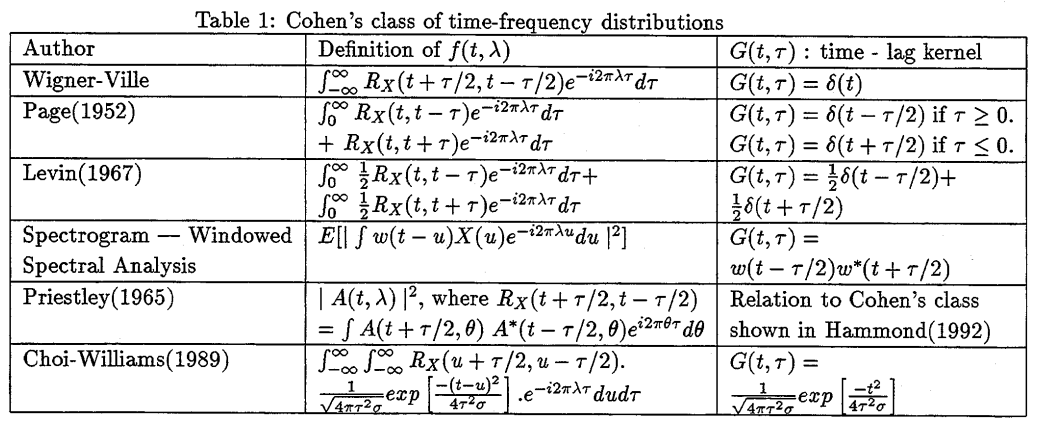
\includegraphics[width=0.9\textwidth]{tabla.png} 
\end{figure}

Dos identidades muy importantes para estimar el espectro son la \textit{equivalencia} entre
el espectro y la funci\'on de autocorrelaci\'on

\begin{equation*}
f(\omega ) = \int R_X(\tau ) e^{-i 2\pi \omega t} d\tau
\end{equation*}

Donde funci\'on de autocorrelaci\'on se ha definido como

\begin{equation*}
R_X(\tau) = E\left[ X(t) X(t+\tau) \right] = \int_0^{\infty} X(t)X(t+\tau) dt
\end{equation*}

[la demostracion es corta, batsa con reescribir una composicion de integrales como convolucion,
la incluire mas tarde]

Por otro lado, se tiene la Identidad de Parseval

\begin{equation*}
\int X^{2}(t) dt = \int f(\omega) d\omega
\end{equation*}

[esta demostracion se basa en la convergencia dominada del modulo de la integral de $X^{2}$ por
la integral del modulo (...), la incluire mas tarde]

%%%%%%%%%%%%%%%%%%%%%%%%%%%%%%%%%%%%%%%%%%%%%%%%%%%%%%%%%%%%%%%%%%%%%%%%%%%%%%%%%%%%%%%%%%%%%%%%%%%

\section{Test Priestley-Subba Rao (PSR)}

(seccion en proceso de re-redaccion)

A muy grosso modo, el test PSR estima localmente  el espectro evolutivo
 y revisa si estad\'isticamente
cambia en el tiempo.

Para ello, usa un estimador para la funci\'on de densidad espectral
que es aproximadamente (asint\'oticamente) insesgado y cuya varianza est\'a
determinada aproximadamente. La estimaci\'on se lleva a cabo en puntos en el tiempo y
la frecuencia tales que en conjunto son aproximadamente no-correlacionados.
Se aplica logaritmo para que la varianza de todos los estimadores sea aproximadamente
la misma (el logaritmo ayuda a), amen que los errores conjuntos tengan una
distribuci\'on cercana a una multinormal con correlaci\'on cero.
Finalmente se aplica una prueba ANOVA de varianza conocida.

%%%%%%%%%%%%%%%%%%%%%%%%%%%%%%%%%%%%%%%%%%%%%%%%%%%%%%%%%%%%%%%%%%%%%%%%%%%%%%%%%%%%%%%%%%%%%%%%%%%

\subsection{El espectro evolutivo}

Consid\'erese un proceso estoc\'astico a tiempo continuo $\{X(t)\}$, tal que
$E[X(t)]=0$ y $E\left[ X^{2}(t)\right] < \infty$ para todo $t$. Es decir que su media es constante
y sus segundos momentos est\'an bien definidos, aunque 
estos \'ultimos pueden cambiar con el tiempo.

Por el momento se supondr\'a que acepta una representaci\'on de la forma

\begin{equation*}
X(t) = \int_{-\pi}^{\pi} A(t ; \omega) e^{i\omega t} \, d Z(\omega)
\end{equation*}

Con $\{ Z(\omega) \}$ una familia de procesos ortogonales\footnote{De nuevo, esto implica que
$\Cov{dZ(\omega_1,dZ(\omega_2))} = \delta(\omega_1,\omega_1) d\omega$, una condici\'on m\'as
d\'ebil que la independencia} tales que

\begin{itemize}
\item $E \left[\abso{ dZ(\omega)}^{2} \right] = d\omega$
\item Para cada $t$ el m\'aximo de $A(t;\cdot)$ se encuentra en 0
\end{itemize}

Esta representaci\'on es an\'aloga a la representaci\'on de Cram\'er para un proceso
estacionario, salvo que se permite que la funci\'on $A$ cambie con el tiempo.
Siguiendo la analog\'ia, se define 
el \textbf{espectro evolutivo} de $\{X(t)\}$, con respecto a la la familia
$\mathcal{F} = \{ e^{i\omega t} A(t; \omega) \}$
 como
 
\begin{equation*}
d F(\omega;t) = \lvert A(t;\omega) \lvert^{2} d\omega
\end{equation*}

Ahora bien, si se supone que $\{X(t)\}$ es estoc\'asticametne diferenciable, entonces
se puede definir una \textbf{funci\'on de densidad espectral}

\begin{equation*}
f(t;\omega) = \lvert A(t;\omega) \lvert^{2}
\end{equation*}

Cabe destaca que si la funci\'on $A(t;\omega)$ fuera constante con respecto a $t$, se obtendr\'ia
un proceso estacionario de orden dos tal cual fue descrito en la secci\'on anterior.

%%%%%%%%%%%%%%%%%%%%%%%%%%%%%%%%%%%%%%%%%%%%%%%%%%%%%%%%%%%%%%%%%%%%%%%%%%%%%%%%%%%%%%%%%%%%%%%%%%%

\subsection{El estimador de doble ventana}

{Estimador de doble ventana (Priestley, 1965 \& 1966)}
Sea una funci\'on $g(u)$ tal que

\begin{equation*}
2\pi \int_{-\infty}^{\infty} \lvert g(u) \lvert^{2} du 
= 
\int_{-\infty}^{\infty} \lvert \Gamma(\omega) \lvert^{2} d\omega
= 1
\end{equation*}

donde se define la \textbf{funci\'on de respuesta ante frecuencia} como

\begin{equation*}
\Gamma(u) = \int_{-\infty}^{\infty} g(u) e^{i u \omega} du
\end{equation*}

Posteriormente se define 

\begin{equation*}
U(t,\omega) = \int_{t-T}^{t} g(u) X_{t-u} e^{i \omega (t-u)} du
\end{equation*}


Sea una funci\'on $w_{T'}(t)$ tal que
\begin{itemize}
\item $w_{T'}(t) \geq 0$ para cualesquiera $t$, $T'$
\item $w_{T'}(t) \rightarrow 0$ cuando $\lvert t \lvert \rightarrow \infty$, para todo $T'$
\item $\displaystyle \int_{-\infty}^{\infty} w_{T'}(t) dt = 1$ para todo $T'$
\item $\displaystyle \int_{-\infty}^{\infty} \left( w_{T'}(t) \right)^{2} dt < \infty$ para todo $T'$
\end{itemize}

Ahora, si se define 
$\displaystyle W_{T'}(\lambda) = \int_{-\infty}^{\infty} e^{-i\lambda t}w_{T'}(t) dt $
\begin{itemize}
\item $\lim_{T'\rightarrow\infty} \left[ T' \int_{t-T}^{t} \lvert W_{T'}(\lambda) \lvert^{2} d\lambda \right] = C$
\end{itemize}


\begin{tcolorbox}
Se define el estimador para $f_t$, con $0 \leq t \leq T$
\begin{equation*}
\widehat{f_t}(\omega) = \int_{t-T}^{t} w_{T'}(u) \lvert U(t-u,\omega) \lvert^{2} du
\end{equation*}
\end{tcolorbox}



%{Modelo AR vs Espectro evolutivo}
%La representaci\'on espectral puede verse como un cambio de coordenadas, al menos puntualmente
%
%\begin{equation*}
%f_t(\omega) = \frac{1}{2 \pi} \sum_{k=-\infty}^{\infty} \gamma_{k,t} e^{-i k \omega}
%\hspace{4em}
%\gamma_{k,t} = \int_{-\pi}^{\pi} f_t(\omega) e^{i k \omega} d\omega
%\end{equation*}
%
%%La dependencia no-unicidad de representaci\'on AR se traduce como
%%la no-unicidad del espectro
%
-----------------------------------------------------------------------

Se define $Y_{i,j} = \log \left( \widehat{f_{t_i}}(\omega_j) \right)$, con las siguientes propiedades

\begin{equation*}
E\left[ Y_{i,j} \right] \thicksim \log \left( f_{t_i}(\omega_j) \right)
\hspace{4em}
\text{Var}\left( {Y\left(t,\omega\right)}\right) \thicksim \sigma^{2}
\end{equation*}

Luego, puede escribirse $Y_{i,j} = \log \left( f_{t_i}(\omega_j) \right) + \varepsilon_{i,j}$,
con $\varepsilon_{i,j}$ va iid

Usando un test ANOVA --de varianza conocida-- se puede saber si $\varepsilon$
\vspace{-1em}
\begin{itemize}
\item Tiene marginales
\item Constante sobre el tiempo
\item Constante sobre las frecuencias
\end{itemize}

\begin{lstlisting}
Priestley-Subba Rao stationarity Test for datos
-----------------------------------------------
Samples used              : 3072 
Samples available         : 3069 
Sampling interval         : 1 
SDF estimator             : Multitaper 
  Number of (sine) tapers : 5 
  Centered                : TRUE 
  Recentered              : FALSE 
Number of blocks          : 11 
Block size                : 279 
Number of blocks          : 11 
p-value for T             : 0.4130131 
p-value for I+R           : 0.1787949 
p-value for T+I+R         : 0.1801353 
\end{lstlisting}

\begin{tabular}{cc}
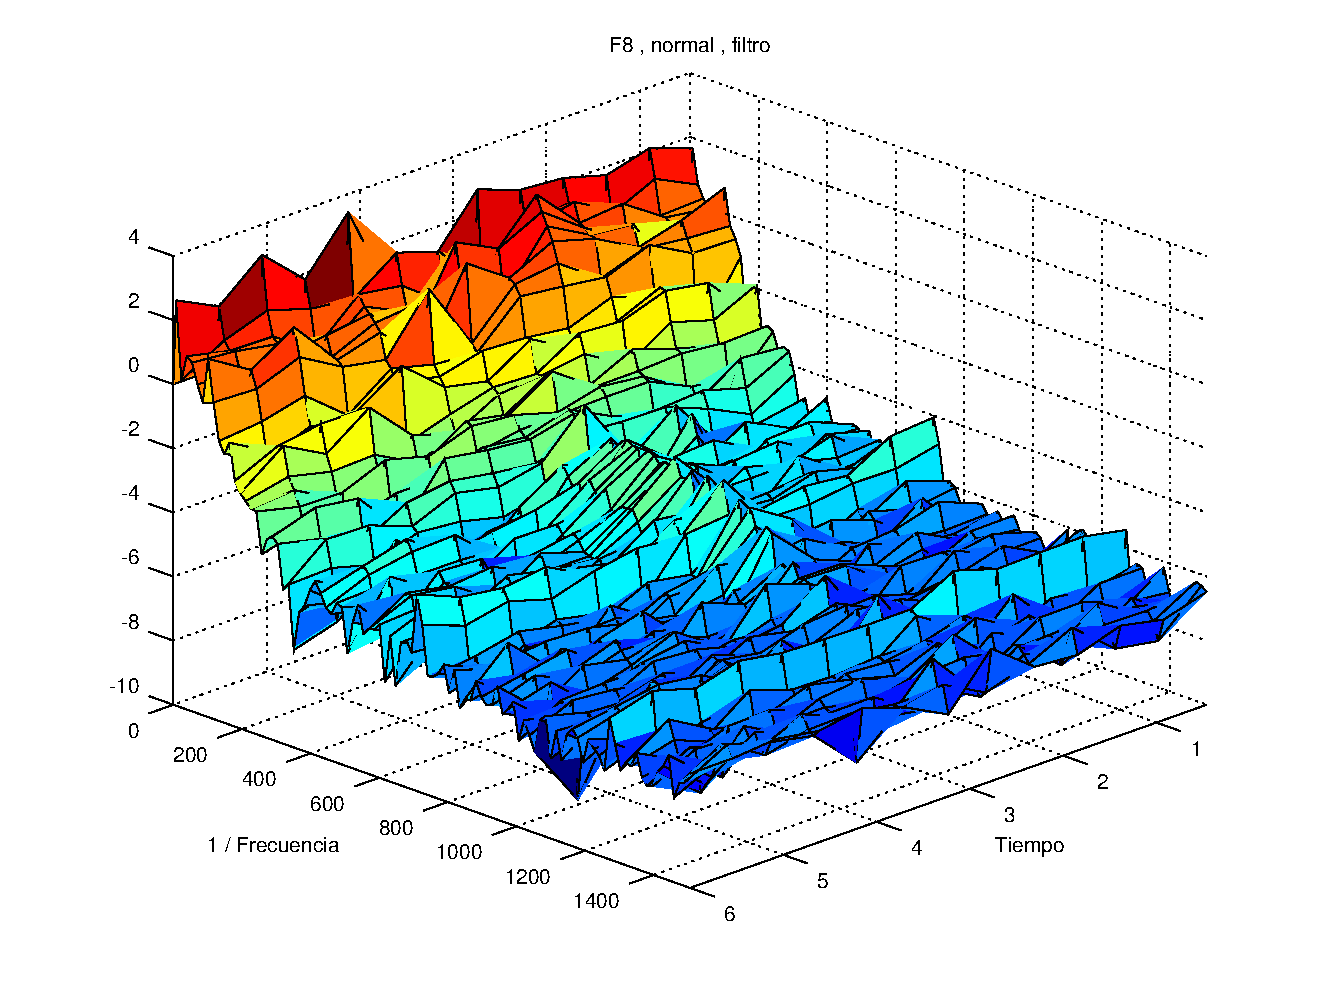
\includegraphics[width=0.5\linewidth]{n8f.pdf} 
&
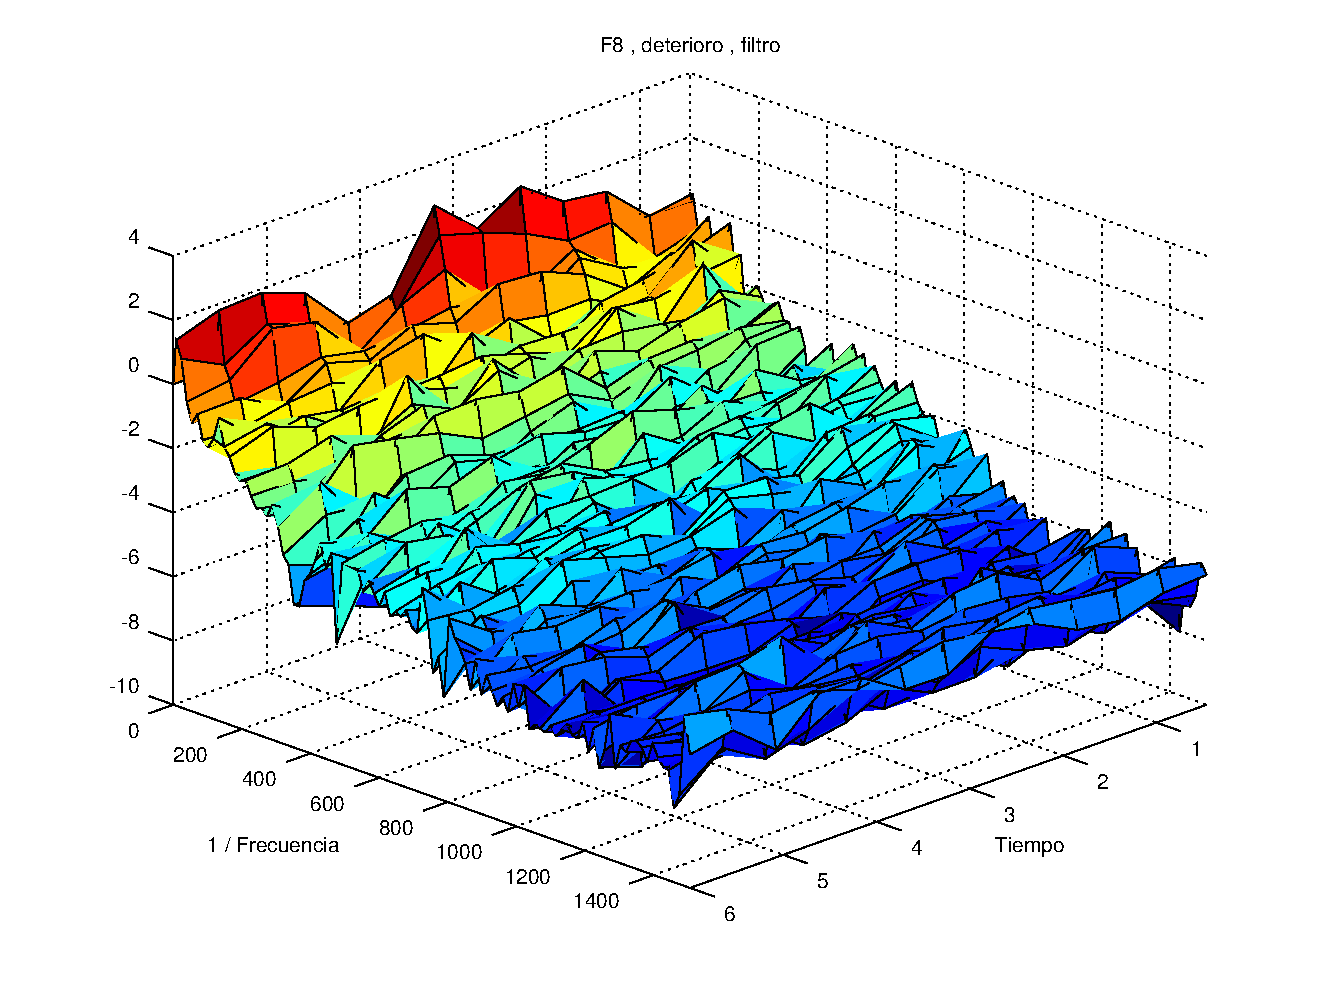
\includegraphics[width=0.5\linewidth]{d8f.pdf} 
\\
\begin{lstlisting}
T      : 0 
I+R    : 5.787895e-09 
T+I+R  : 0 
\end{lstlisting}
&
\begin{lstlisting}
T      : 0.00332259 
I+R    : 0.03502537 
T+I+R  : 0.01598073 
\end{lstlisting}
\end{tabular}

%%%%%%%%%%%%%%%%%%%%%%%%%%%%%%%%%%%%%%%%%%%%%%%%%%%%%%%%%%%%%%%%%%%%%%%%%%%%%%%%%%%%%%%%%%%%%%%%%%%
%%%%%%%%%%%%%%%%%%%%%%%%%%%%%%%%%%%%%%%%%%%%%%%%%%%%%%%%%%%%%%%%%%%%%%%%%%%%%%%%%%%%%%%%%%%%%%%%%%%